\documentclass[11pt]{article}

\usepackage[top=0.45in,bottom=0.65in,left=0.7in,right=0.7in]{geometry}
\usepackage{graphicx}
\usepackage{booktabs}
\usepackage{amsmath}
\usepackage{caption}
\usepackage{enumitem}
\usepackage{float}
\usepackage{titlesec}
\usepackage{url}

\captionsetup{font=small,skip=3pt}
\setlength{\parindent}{1em}
\setlength{\parskip}{0.08em}
\setlist{nosep,leftmargin=*}
\titlespacing*{\section}{0pt}{0.55em}{0.25em}

\makeatletter
\renewcommand{\maketitle}{
    \begin{center}
    \vspace*{-2.4em}
    {\Large\bfseries \@title \par}
    \vspace{0.15em}
    {\normalsize \@author \par}
    \vspace{0.08em}
    {\footnotesize GitHub: \url{https://github.com/Lu-Shen939/CS5782-Final-Report---vit-attention-initialization-reproduction} \par}
    \vspace{-0.35em}
    \end{center}
}
\makeatother

\title{From Mimetic to Structured Initialization:\\[-0.15em] Reproducing Attention Biases for Small-Data Vision Transformers}
\author{Lu Shen (ls2244), Xuanbo Jia (xj256), Yichen Li (yl3938)}
\date{}

\begin{document}
\maketitle

\section{Introduction}
Vision Transformers (ViTs) can perform very well at scale, but they are often
less data-efficient than convolutional neural networks when trained from scratch
on small image datasets.  CNNs contain locality and translation bias by design,
while vanilla ViTs must learn spatial structure through attention.  This project
studies whether useful spatial bias can be injected only through initialization,
without changing the ViT architecture.

We reproduce and connect two related ideas.  Mimetic initialization observes
that pretrained transformers contain structured attention-weight statistics,
especially diagonal patterns, and initializes a new model to mimic those
statistics.  Structured initialization goes further by directly programming the
initial attention maps to resemble local convolutional impulse filters.  Our
goal is to test whether these initialization methods improve CIFAR-10 and
CIFAR-100 performance in full-data and low-data settings.

\section{Chosen Result}
The chosen result is the accuracy and attention-structure comparison among
three ViT initializations: Default, Mimetic, and Structured.  This combines the
main claims of the two papers: Mimetic should improve training by copying
pretrained-like self-attention statistics, while Structured should improve
small-data learning by explicitly imposing local attention at initialization.
We therefore reproduce both quantitative accuracy trends and qualitative
attention-map structure.  The quantitative result is summarized later in
Figure~\ref{fig:combined-accuracy}, and the attention-map component is shown in
Figure~\ref{fig:attention-maps}.

\begin{figure}[H]
    \centering
    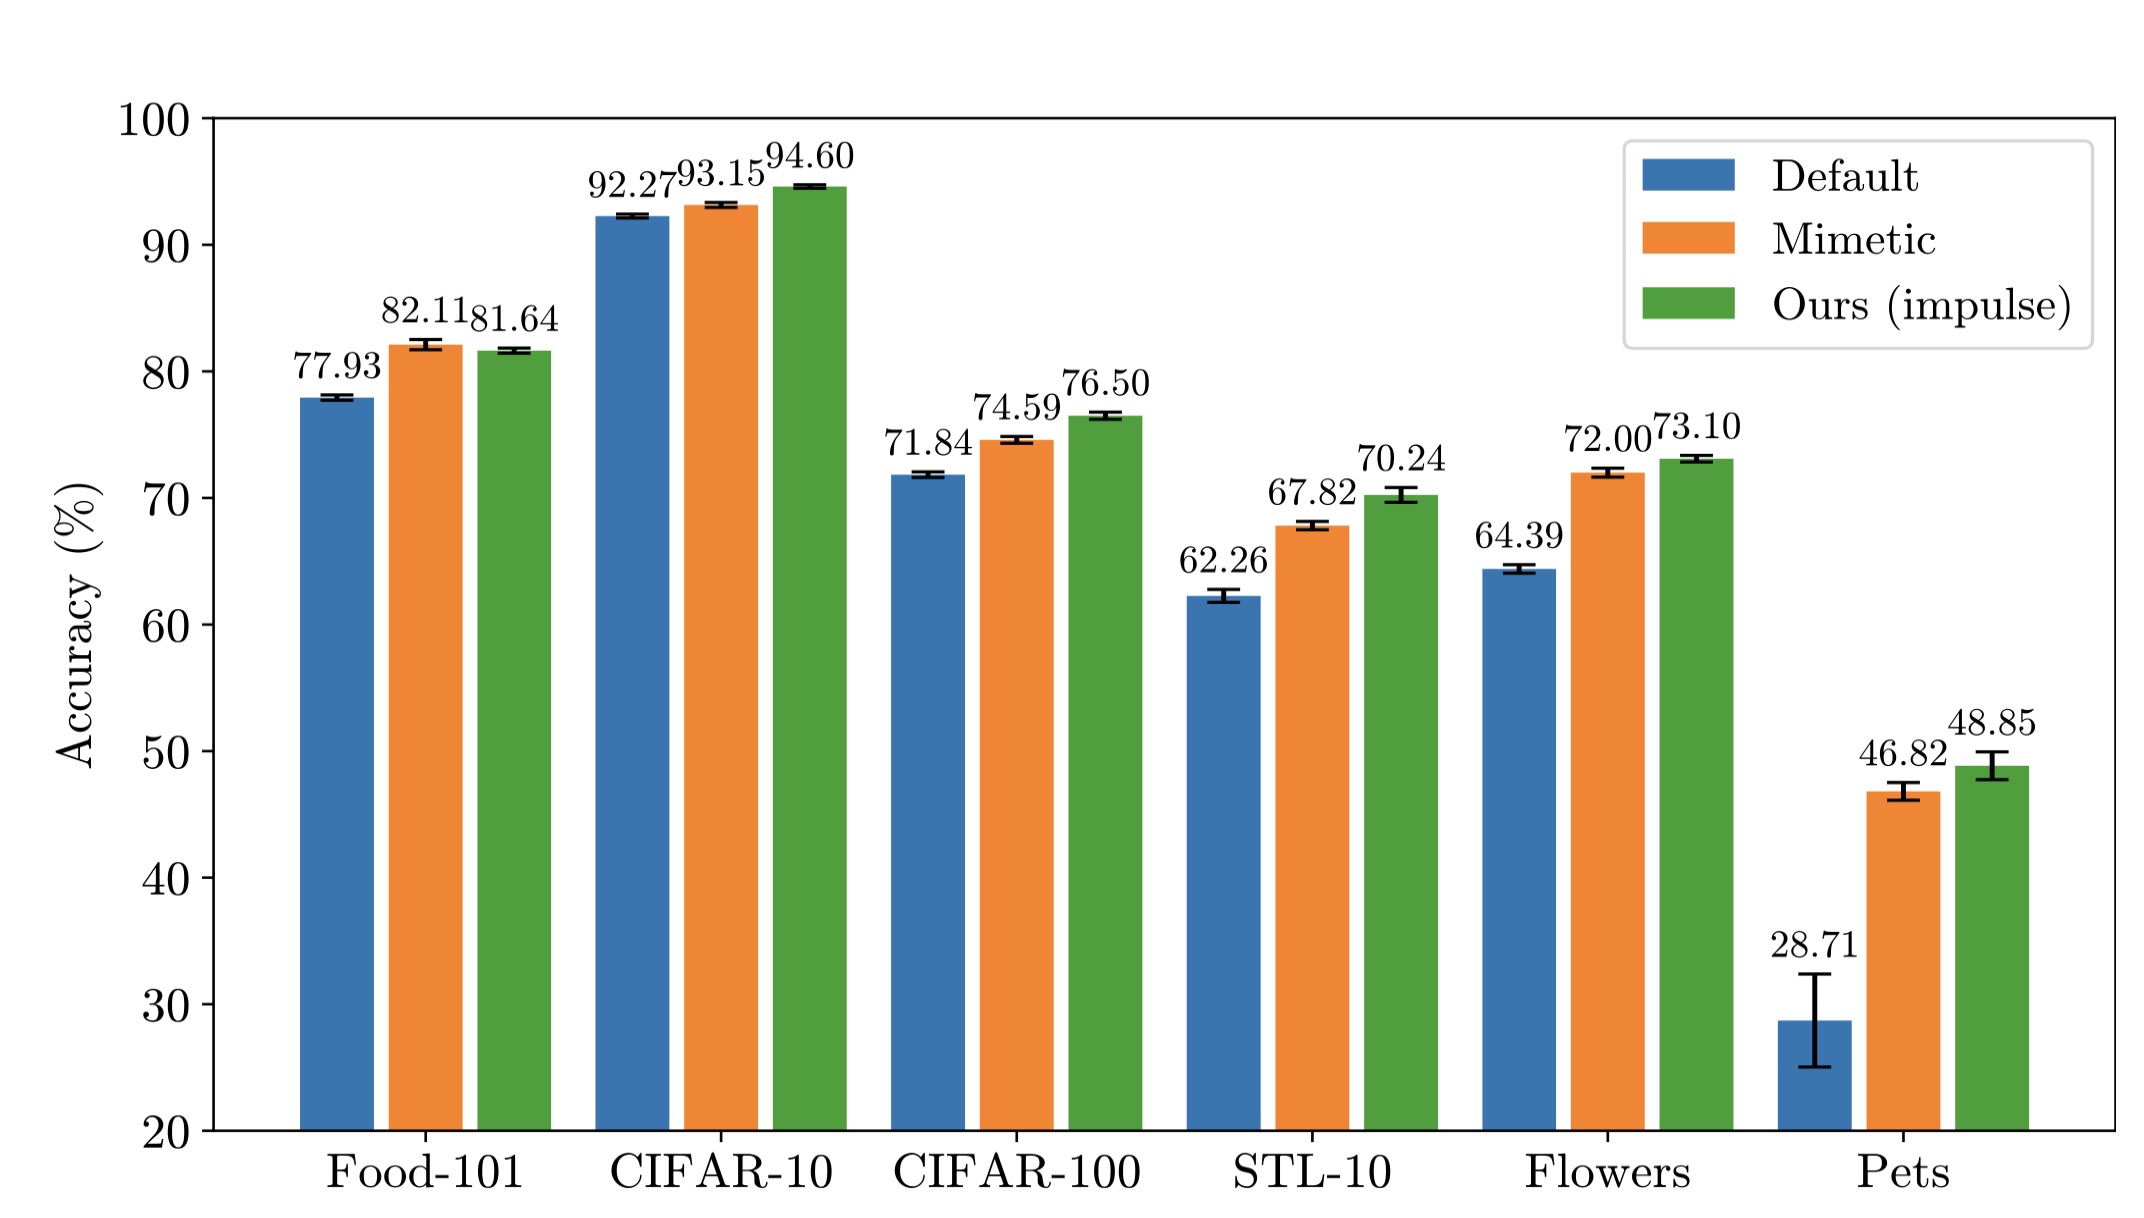
\includegraphics[width=0.82\linewidth]{figures/fig_paper_reported_accuracy.png}
    \caption{
    Original paper's reported ViT-Tiny accuracy comparison across datasets
    (adapted from Zheng et al., 2025).
    This is the quantitative trend we use as the target for reproduction:
    Default, Mimetic, and Structured/Impulse initialization are compared under
    the same model family.
    }
    \label{fig:paper-reported-accuracy}
\end{figure}

\section{Methodology}
We reimplemented the experiment in PyTorch using a ViT-Tiny style model from
\texttt{timm}: 12 transformer layers, embedding dimension 192, 3 attention
heads, image size $32\times32$, and patch size 4.  We evaluated CIFAR-10 and
CIFAR-100 with full training data, plus 10\% and 25\% training-subset settings
to test the small-data regime.  The compared methods were default truncated
normal initialization, Mimetic initialization, and Structured impulse
initialization.

We used the official training recipe with AdamW, learning rate $2\times10^{-3}$,
weight decay 0.05, cosine scheduling, 10 warmup epochs, RandAugment, Mixup,
CutMix, label smoothing, random erasing, and stochastic depth.  Full-data runs
used batch size 1024 for 300 epochs on CIFAR-10 and 250 epochs on CIFAR-100;
low-data runs used batch size 512 for 150 epochs on a Colab A100.  Mimetic
initializes attention projections toward pretrained-like products
($QK\!\approx\!I$, $VO\!\approx\!-I$), while Structured optimizes Q/K from
positional embeddings so initial attention approximates sparse local impulse
filters.  We report best top-1 accuracy, training curves, seed stability, and
trained patch-to-patch attention maps.

% Requires: \usepackage{graphicx,booktabs}

\section{Results and Analysis}

Figure~\ref{fig:combined-accuracy} summarizes our reproduced results across six
settings: full CIFAR-10/100, 10\% CIFAR-10/100, and 25\% CIFAR-10/100.  Compared
with the original paper trend in Figure~\ref{fig:paper-reported-accuracy}, our
absolute numbers are lower but the method ordering is similar: both
initialization methods improve over the default ViT initialization, and
Structured initialization is usually strongest.  On full CIFAR-10, accuracy
improves from 89.12\% for Default to 91.99\% for Mimetic and 92.47\% for
Structured.  On full CIFAR-100, the same ordering appears: 67.95\%, 72.67\%,
and 73.40\%.  This suggests that attention initialization is a useful way to
inject inductive bias without changing the ViT architecture.

\begin{figure}[H]
    \centering
    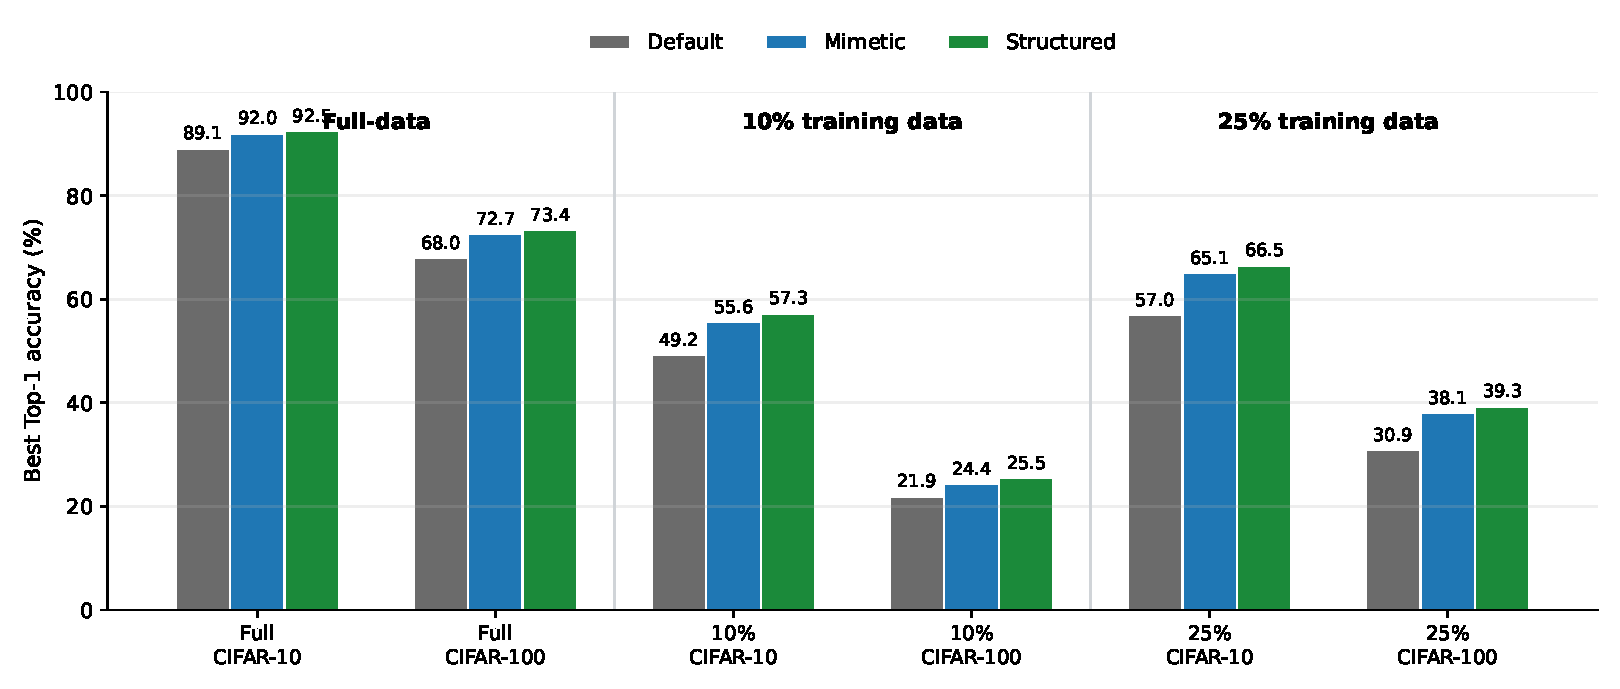
\includegraphics[width=\linewidth]{figures/fig_results_accuracy_combined.pdf}
    \caption{
    Best top-1 accuracy across full-data and low-data settings.  Structured
    initialization gives the best result in most settings, while Mimetic also
    consistently improves over the default baseline.
    }
    \label{fig:combined-accuracy}
\end{figure}

The advantage is especially visible in the low-data experiments.  With 10\% of
CIFAR-10, Mimetic improves over Default by 6.35 points, while Structured improves
by 8.06 points.  With 25\% of CIFAR-10, the gains become 8.17 and 9.58 points.
For CIFAR-100, Structured also improves over Default by 3.55 points at 10\% data
and 8.42 points at 25\% data.  These results support the small-data motivation:
when less supervision is available, a spatial attention prior helps the model
avoid learning locality completely from scratch.

Qualitatively, Mimetic helps by copying pretrained-like self-attention
statistics, while Structured is more explicit: it initializes query/key
attention to resemble local convolutional impulse filters.  The trained
attention maps in Figure~\ref{fig:attention-maps} provide a visual check:
Mimetic and Structured runs show clearer diagonal/local patterns than a purely
default initialization.  The L1/L6/L12 comparison also follows the original
paper visualization, where the impulse initialization produces strong local
diagonal attention.

\begin{figure}[H]
    \centering
    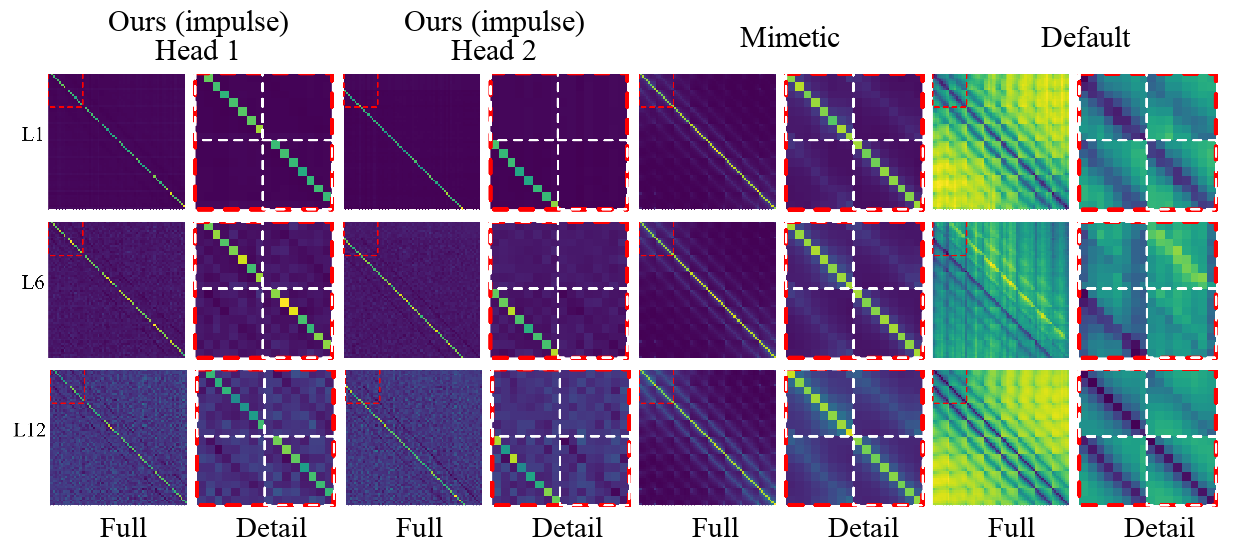
\includegraphics[width=\linewidth]{figures/fig_paper_attention_maps_l1_l6_l12.png}
    \vspace{0.2em}

    {\small (a) Original paper attention-map figure at L1, L6, and L12.}
    \vspace{0.45em}

    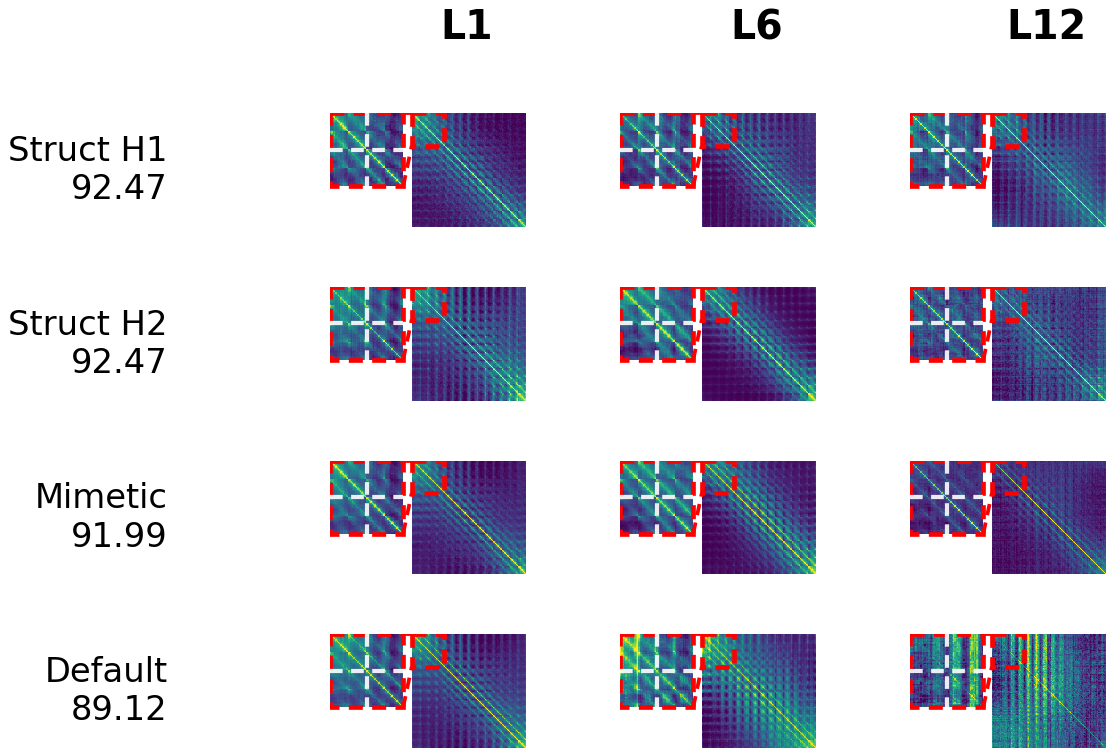
\includegraphics[width=0.86\linewidth]{figures/fig_attention_maps_cifar10.png}
    \vspace{0.2em}

    {\small (b) Our trained CIFAR-10 seed-0 checkpoint attention maps.}
    \caption{
    Attention-map comparison.  Both panels show patch-to-patch attention
    patterns at L1/L6/L12; brighter diagonal structures indicate stronger local
    patch attention.
    }
    \label{fig:attention-maps}
\end{figure}

Our absolute accuracies are still below the full results reported in the
original papers.  A likely reason is that our reproduction used a shorter
few-hundred-epoch training budget, fewer seed/hyperparameter sweeps, and an
independent reimplementation.  Therefore, the most important reproduced result
is the relative pattern rather than exact matching: Default $<$ Mimetic $<$
Structured in most full-data and low-data settings.

\begin{table}[H]
\centering
\small
\caption{CIFAR-10 seed stability under a common 250-epoch budget.}
\label{tab:seed-stability}
\begin{tabular}{lrrrr}
\toprule
Initialization & Seed 0 & Seed 1 & Seed 2 & Mean $\pm$ Std \\
\midrule
Default & 88.20 & 87.72 & 87.44 & 87.79 $\pm$ 0.38 \\
Mimetic & 91.32 & 91.03 & 90.42 & 90.92 $\pm$ 0.46 \\
Structured & 91.85 & 90.90 & 89.92 & 90.89 $\pm$ 0.97 \\
\bottomrule
\end{tabular}
\end{table}


The seed study adds an important caveat.  On CIFAR-10 at 250 epochs, Structured
is best for seed 0, but has higher variance across seeds (0.97 std) than Mimetic
(0.46 std) or Default (0.38 std).  This suggests that the stronger structured
locality prior can be more sensitive to the early training trajectory.  When the
prior aligns well with the data order and augmentation noise, it helps; when it
does not, the model may need more training to adapt from local attention toward
more task-specific attention patterns.

Figure~\ref{fig:training-curves} shows the corresponding training curves from
the exported logs.  Mimetic and Structured generally rise faster and end higher
than Default, so their advantage appears during optimization rather than only at
the final checkpoint.


\section{Reflections}
This project was successful in reproducing the main qualitative conclusion of
the two papers: better attention initialization can improve small-data ViT
training without modifying the architecture.  The clearest result is that
Mimetic initialization is a reliable improvement over the default baseline, and
Structured initialization usually provides the largest gain, especially in
low-data settings.

The main limitation is that our absolute accuracies are below the original
reported results.  This is expected for a course-scale reproduction because we
used a smaller compute budget, fewer seeds, and a simplified training sweep.
The seed study also shows that Structured initialization is not uniformly stable:
its stronger locality bias can improve data efficiency, but may also increase
sensitivity to the exact run.  With more time, we would train for the full
original schedule, sweep learning-rate and augmentation settings, and evaluate
more seeds to separate method-level gains from run-to-run variance.

\section{References}
\small
\begin{enumerate}[itemsep=0pt,topsep=0pt,parsep=0pt]
    \item A. Trockman and J. Z. Kolter. \textit{Mimetic Initialization of
    Self-Attention Layers}. ICML, 2023.
    \item J. Zheng et al. \textit{Structured Initialization for Vision
    Transformers}. NeurIPS, 2025.
    \item A. Krizhevsky. \textit{Learning Multiple Layers of Features from Tiny
    Images}. Technical report, 2009. CIFAR-10/CIFAR-100.
    \item A. Paszke et al. \textit{PyTorch: An Imperative Style,
    High-Performance Deep Learning Library}. NeurIPS, 2019.
    \item R. Wightman. \textit{PyTorch Image Models / timm}. GitHub repository,
    2019.
    \item C. R. Harris et al. \textit{Array Programming with NumPy}. Nature,
    2020; J. D. Hunter. \textit{Matplotlib}. Computing in Science \&
    Engineering, 2007.
\end{enumerate}
\normalsize

\vspace{-0.25em}
\begin{center}
\begin{minipage}{0.34\linewidth}
    \centering
    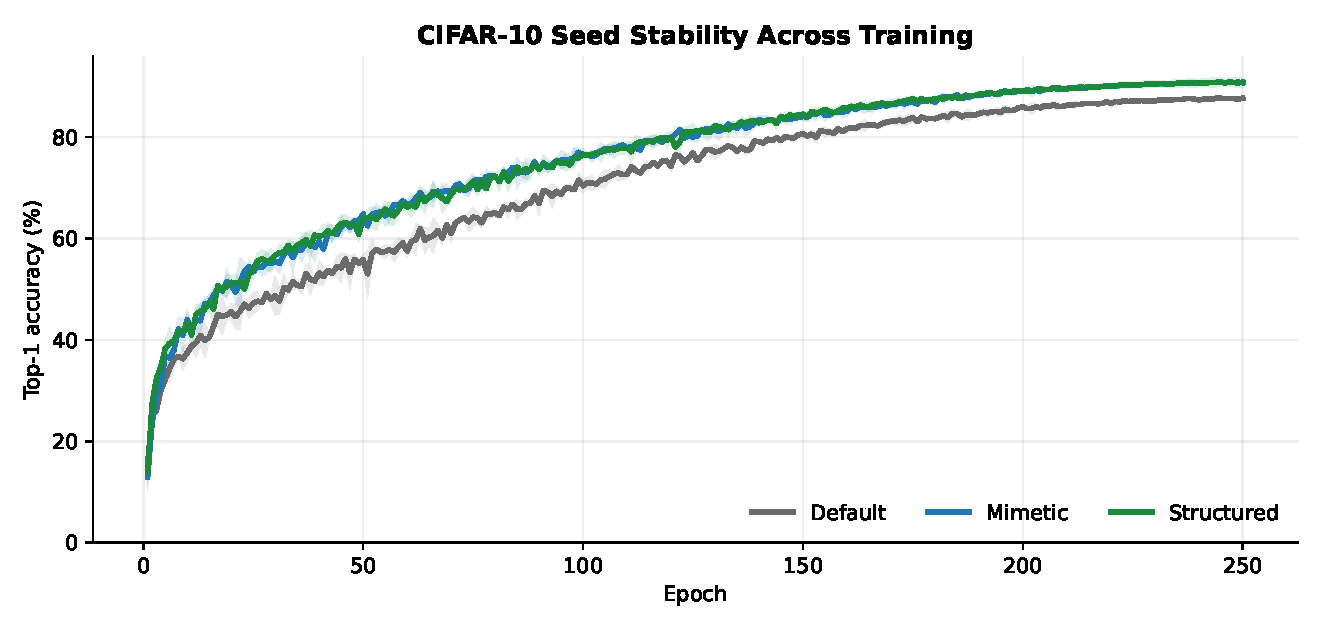
\includegraphics[width=\linewidth]{figures/fig_seed_stability_curve.pdf}
    \captionof{figure}{CIFAR-10 seed stability over seeds 0, 1, and 2.}
    \label{fig:seed-stability}
\end{minipage}
\hfill
\begin{minipage}{0.62\linewidth}
    \centering
    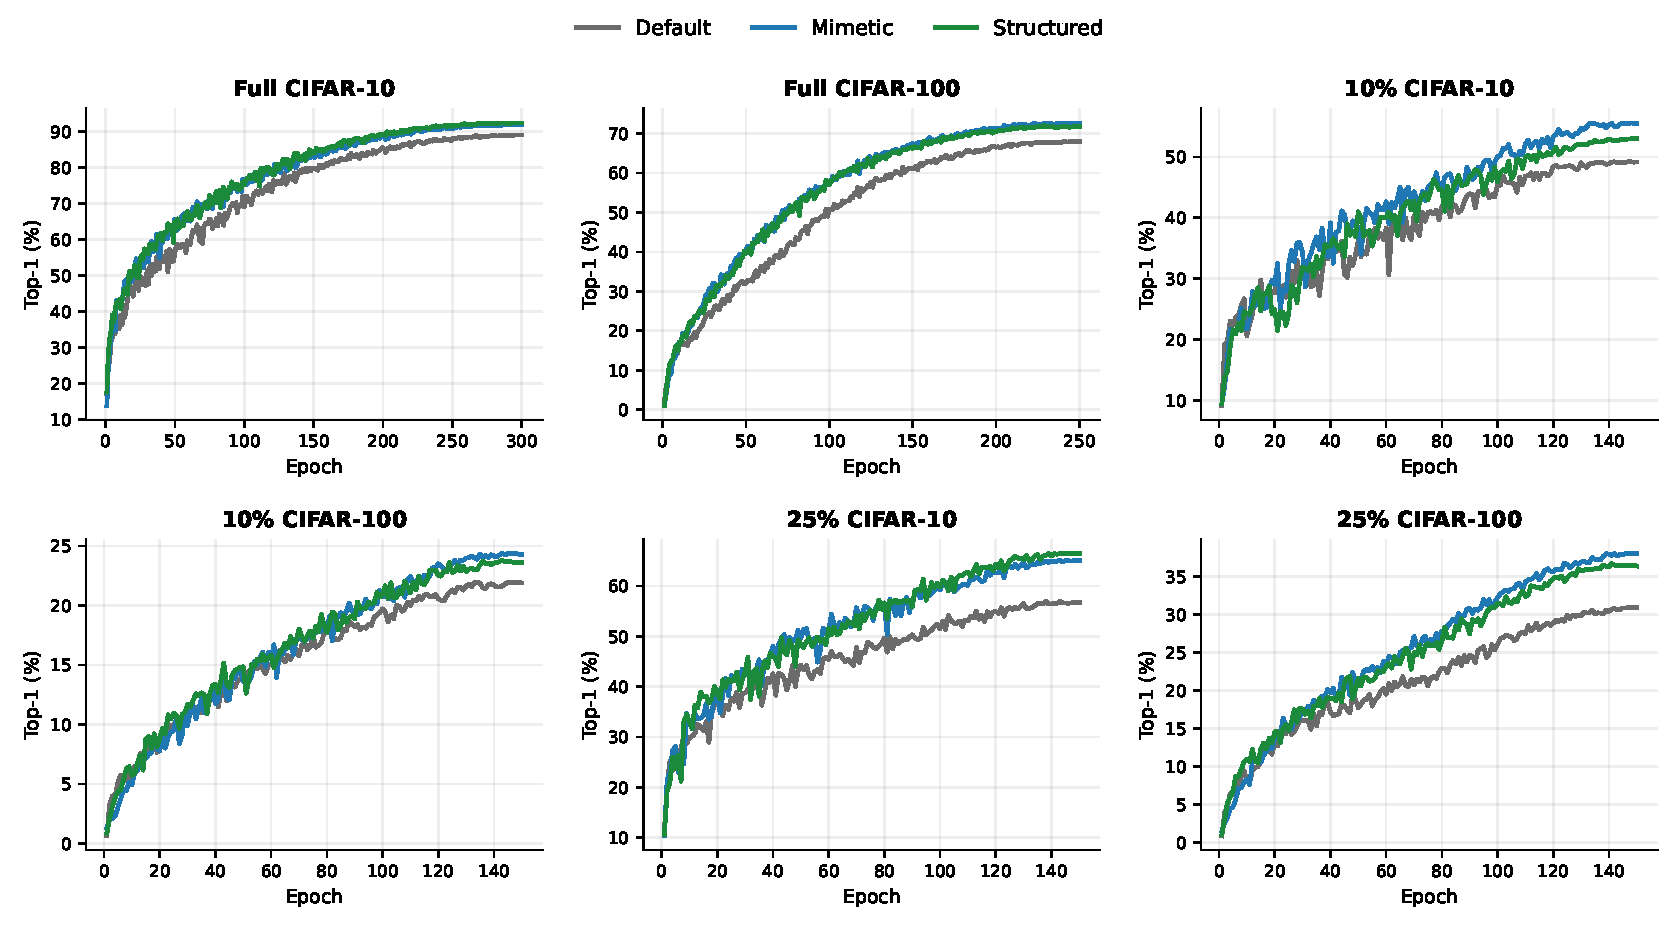
\includegraphics[width=\linewidth]{figures/fig_training_curves_grid.pdf}
    \captionof{figure}{Training curves for the six evaluated settings.}
    \label{fig:training-curves}
\end{minipage}
\end{center}

\end{document}
